\documentclass{standalone}
\usepackage{tikz}
\usetikzlibrary{patterns, positioning}


\begin{document}
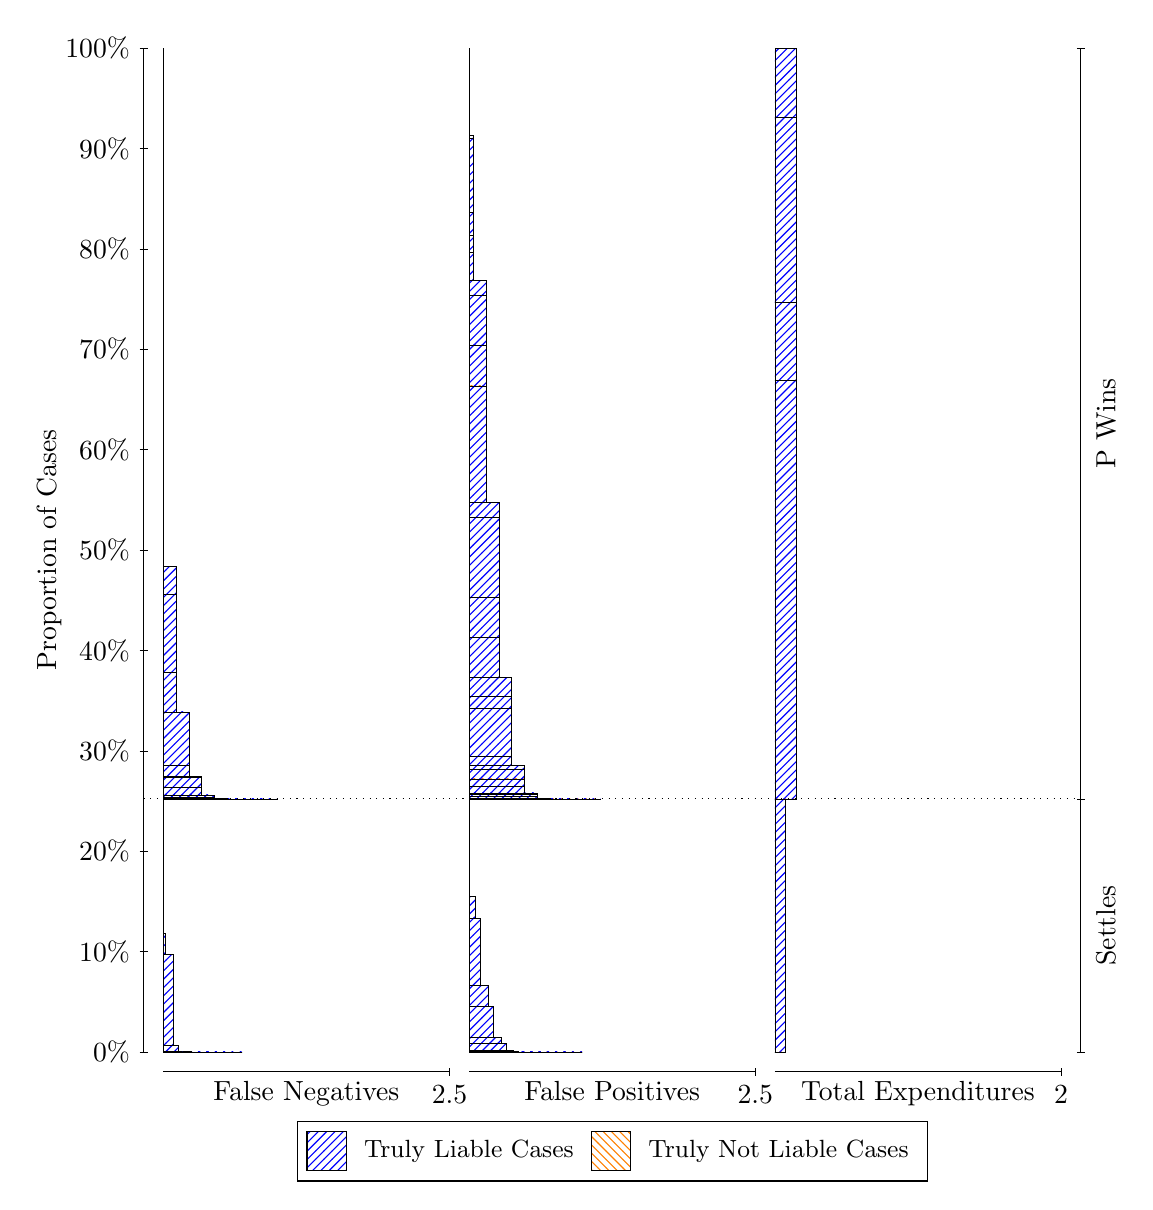
\begin{tikzpicture}
\draw[black, very thin] (1.5,1.75) -- (1.5,14.5);
\node[rotate=90, text=black, anchor=center] at (0.3, 8.125) {Proportion of Cases};
\draw[black, very thin] (1.45,1.75) -- (1.55,1.75);
\node[text=black, anchor=east] at (1.45, 1.75) {0\%};
\draw[black, very thin] (1.45,3.025) -- (1.55,3.025);
\node[text=black, anchor=east] at (1.45, 3.025) {10\%};
\draw[black, very thin] (1.45,4.3) -- (1.55,4.3);
\node[text=black, anchor=east] at (1.45, 4.3) {20\%};
\draw[black, very thin] (1.45,5.575) -- (1.55,5.575);
\node[text=black, anchor=east] at (1.45, 5.575) {30\%};
\draw[black, very thin] (1.45,6.85) -- (1.55,6.85);
\node[text=black, anchor=east] at (1.45, 6.85) {40\%};
\draw[black, very thin] (1.45,8.125) -- (1.55,8.125);
\node[text=black, anchor=east] at (1.45, 8.125) {50\%};
\draw[black, very thin] (1.45,9.4) -- (1.55,9.4);
\node[text=black, anchor=east] at (1.45, 9.4) {60\%};
\draw[black, very thin] (1.45,10.675) -- (1.55,10.675);
\node[text=black, anchor=east] at (1.45, 10.675) {70\%};
\draw[black, very thin] (1.45,11.95) -- (1.55,11.95);
\node[text=black, anchor=east] at (1.45, 11.95) {80\%};
\draw[black, very thin] (1.45,13.225) -- (1.55,13.225);
\node[text=black, anchor=east] at (1.45, 13.225) {90\%};
\draw[black, very thin] (1.45,14.5) -- (1.55,14.5);
\node[text=black, anchor=east] at (1.45, 14.5) {100\%};

\draw[black, very thin] (13.4,1.75) -- (13.4,14.5);
\draw[black, very thin] (13.35,1.75) -- (13.45,1.75);
\node[anchor=west] at (13.35, 1.75) {};
\draw[black, very thin] (13.35,4.9648) -- (13.45,4.9648);
\node[anchor=west] at (13.35, 4.9648) {};
\draw[black, very thin] (13.35,14.5) -- (13.45,14.5);
\node[anchor=west] at (13.35, 14.5) {};

\draw[black, very thin, pattern color=blue, pattern=north east lines] (1.75,1.75) rectangle (2.7492,1.75);
\draw[black, very thin, pattern color=blue, pattern=north east lines] (1.75,1.75) rectangle (2.5877,1.75);
\draw[black, very thin, pattern color=blue, pattern=north east lines] (1.75,1.75) rectangle (2.4262,1.75);
\draw[black, very thin, pattern color=blue, pattern=north east lines] (1.75,1.75) rectangle (2.3132,1.75);
\draw[black, very thin, pattern color=blue, pattern=north east lines] (1.75,1.75) rectangle (2.2647,1.7503);
\draw[black, very thin, pattern color=blue, pattern=north east lines] (1.75,1.7503) rectangle (2.1517,1.7503);
\draw[black, very thin, pattern color=blue, pattern=north east lines] (1.75,1.7503) rectangle (2.1032,1.7581);
\draw[black, very thin, pattern color=blue, pattern=north east lines] (1.75,1.7581) rectangle (1.9902,1.7581);
\draw[black, very thin, pattern color=blue, pattern=north east lines] (1.75,1.7581) rectangle (1.9418,1.8376);
\draw[black, very thin, pattern color=blue, pattern=north east lines] (1.75,1.8376) rectangle (1.8772,2.9894);
\draw[black, very thin, pattern color=blue, pattern=north east lines] (1.75,2.9894) rectangle (1.8287,2.9894);
\draw[black, very thin, pattern color=blue, pattern=north east lines] (1.75,2.9894) rectangle (1.7803,3.2613);
\draw[black, very thin, pattern color=orange, pattern=north west lines] (1.75,3.2613) rectangle (1.75,3.2613);
\draw[black, very thin, pattern color=blue, pattern=north east lines] (1.75,3.2613) rectangle (1.75,4.9648);
\draw[black, very thin, pattern color=blue, pattern=north east lines] (1.75,4.9648) rectangle (3.2033,4.9648);
\draw[black, very thin, pattern color=blue, pattern=north east lines] (1.75,4.9648) rectangle (3.0419,4.9648);
\draw[black, very thin, pattern color=blue, pattern=north east lines] (1.75,4.9648) rectangle (2.8804,4.9648);
\draw[black, very thin, pattern color=blue, pattern=north east lines] (1.75,4.9648) rectangle (2.8804,4.9648);
\draw[black, very thin, pattern color=blue, pattern=north east lines] (1.75,4.9648) rectangle (2.7189,4.965);
\draw[black, very thin, pattern color=blue, pattern=north east lines] (1.75,4.965) rectangle (2.7189,4.9652);
\draw[black, very thin, pattern color=blue, pattern=north east lines] (1.75,4.9652) rectangle (2.5574,4.9702);
\draw[black, very thin, pattern color=blue, pattern=north east lines] (1.75,4.9702) rectangle (2.3959,4.9887);
\draw[black, very thin, pattern color=blue, pattern=north east lines] (1.75,4.9887) rectangle (2.3959,5.0149);
\draw[black, very thin, pattern color=blue, pattern=north east lines] (1.75,5.0149) rectangle (2.2344,5.1056);
\draw[black, very thin, pattern color=blue, pattern=north east lines] (1.75,5.1056) rectangle (2.2344,5.2352);
\draw[black, very thin, pattern color=blue, pattern=north east lines] (1.75,5.2352) rectangle (2.2344,5.2542);
\draw[black, very thin, pattern color=blue, pattern=north east lines] (1.75,5.2542) rectangle (2.073,5.394);
\draw[black, very thin, pattern color=blue, pattern=north east lines] (1.75,5.394) rectangle (2.073,6.0694);
\draw[black, very thin, pattern color=blue, pattern=north east lines] (1.75,6.0694) rectangle (1.9115,6.5728);
\draw[black, very thin, pattern color=blue, pattern=north east lines] (1.75,6.5728) rectangle (1.9115,7.5587);
\draw[black, very thin, pattern color=blue, pattern=north east lines] (1.75,7.5587) rectangle (1.9115,7.9176);
\draw[black, very thin, pattern color=orange, pattern=north west lines] (1.75,7.9176) rectangle (1.75,7.9176);
\draw[black, very thin, pattern color=blue, pattern=north east lines] (1.75,7.9176) rectangle (1.75,14.5);
\draw[black, very thin, pattern color=orange, pattern=north west lines] (5.6333,1.75) rectangle (7.0685,1.75);
\draw[black, very thin, pattern color=blue, pattern=north east lines] (5.6333,1.75) rectangle (7.0685,1.75);
\draw[black, very thin, pattern color=blue, pattern=north east lines] (5.6333,1.75) rectangle (6.907,1.75);
\draw[black, very thin, pattern color=blue, pattern=north east lines] (5.6333,1.75) rectangle (6.7455,1.75);
\draw[black, very thin, pattern color=orange, pattern=north west lines] (5.6333,1.75) rectangle (6.6325,1.75);
\draw[black, very thin, pattern color=blue, pattern=north east lines] (5.6333,1.75) rectangle (6.6325,1.75);
\draw[black, very thin, pattern color=blue, pattern=north east lines] (5.6333,1.75) rectangle (6.5841,1.75);
\draw[black, very thin, pattern color=blue, pattern=north east lines] (5.6333,1.75) rectangle (6.471,1.75);
\draw[black, very thin, pattern color=blue, pattern=north east lines] (5.6333,1.75) rectangle (6.4226,1.7503);
\draw[black, very thin, pattern color=blue, pattern=north east lines] (5.6333,1.7503) rectangle (6.3095,1.7503);
\draw[black, very thin, pattern color=blue, pattern=north east lines] (5.6333,1.7503) rectangle (6.2611,1.7581);
\draw[black, very thin, pattern color=orange, pattern=north west lines] (5.6333,1.7581) rectangle (6.1965,1.7581);
\draw[black, very thin, pattern color=blue, pattern=north east lines] (5.6333,1.7581) rectangle (6.1965,1.7695);
\draw[black, very thin, pattern color=blue, pattern=north east lines] (5.6333,1.7695) rectangle (6.1481,1.7695);
\draw[black, very thin, pattern color=blue, pattern=north east lines] (5.6333,1.7695) rectangle (6.0996,1.8544);
\draw[black, very thin, pattern color=blue, pattern=north east lines] (5.6333,1.8544) rectangle (6.035,1.9391);
\draw[black, very thin, pattern color=blue, pattern=north east lines] (5.6333,1.9391) rectangle (5.9866,1.9391);
\draw[black, very thin, pattern color=blue, pattern=north east lines] (5.6333,1.9391) rectangle (5.9381,2.327);
\draw[black, very thin, pattern color=blue, pattern=north east lines] (5.6333,2.327) rectangle (5.8735,2.5999);
\draw[black, very thin, pattern color=blue, pattern=north east lines] (5.6333,2.5999) rectangle (5.8251,2.6);
\draw[black, very thin, pattern color=blue, pattern=north east lines] (5.6333,2.6) rectangle (5.7766,3.4535);
\draw[black, very thin, pattern color=blue, pattern=north east lines] (5.6333,3.4535) rectangle (5.7121,3.7254);
\draw[black, very thin, pattern color=blue, pattern=north east lines] (5.6333,3.7254) rectangle (5.6636,3.7254);
\draw[black, very thin, pattern color=blue, pattern=north east lines] (5.6333,3.7254) rectangle (5.6333,4.9648);
\draw[black, very thin, pattern color=orange, pattern=north west lines] (5.6333,4.9648) rectangle (7.3047,4.9648);
\draw[black, very thin, pattern color=blue, pattern=north east lines] (5.6333,4.9648) rectangle (7.3047,4.9648);
\draw[black, very thin, pattern color=orange, pattern=north west lines] (5.6333,4.9648) rectangle (7.1432,4.9648);
\draw[black, very thin, pattern color=blue, pattern=north east lines] (5.6333,4.9648) rectangle (7.1432,4.9648);
\draw[black, very thin, pattern color=orange, pattern=north west lines] (5.6333,4.9648) rectangle (6.9817,4.9648);
\draw[black, very thin, pattern color=blue, pattern=north east lines] (5.6333,4.9648) rectangle (6.9817,4.9648);
\draw[black, very thin, pattern color=blue, pattern=north east lines] (5.6333,4.9648) rectangle (6.9817,4.9648);
\draw[black, very thin, pattern color=blue, pattern=north east lines] (5.6333,4.9648) rectangle (6.9817,4.9649);
\draw[black, very thin, pattern color=orange, pattern=north west lines] (5.6333,4.9649) rectangle (6.8202,4.9649);
\draw[black, very thin, pattern color=blue, pattern=north east lines] (5.6333,4.9649) rectangle (6.8202,4.9654);
\draw[black, very thin, pattern color=blue, pattern=north east lines] (5.6333,4.9654) rectangle (6.8202,4.9655);
\draw[black, very thin, pattern color=orange, pattern=north west lines] (5.6333,4.9655) rectangle (6.6587,4.9655);
\draw[black, very thin, pattern color=blue, pattern=north east lines] (5.6333,4.9655) rectangle (6.6587,4.9692);
\draw[black, very thin, pattern color=blue, pattern=north east lines] (5.6333,4.9692) rectangle (6.6587,4.9737);
\draw[black, very thin, pattern color=blue, pattern=north east lines] (5.6333,4.9737) rectangle (6.4973,4.9942);
\draw[black, very thin, pattern color=orange, pattern=north west lines] (5.6333,4.9942) rectangle (6.4973,4.9942);
\draw[black, very thin, pattern color=blue, pattern=north east lines] (5.6333,4.9942) rectangle (6.4973,5.0201);
\draw[black, very thin, pattern color=blue, pattern=north east lines] (5.6333,5.0201) rectangle (6.4973,5.0409);
\draw[black, very thin, pattern color=blue, pattern=north east lines] (5.6333,5.0409) rectangle (6.3358,5.1263);
\draw[black, very thin, pattern color=blue, pattern=north east lines] (5.6333,5.1263) rectangle (6.3358,5.2185);
\draw[black, very thin, pattern color=orange, pattern=north west lines] (5.6333,5.2185) rectangle (6.3358,5.2185);
\draw[black, very thin, pattern color=blue, pattern=north east lines] (5.6333,5.2185) rectangle (6.3358,5.3403);
\draw[black, very thin, pattern color=blue, pattern=north east lines] (5.6333,5.3403) rectangle (6.3358,5.3882);
\draw[black, very thin, pattern color=blue, pattern=north east lines] (5.6333,5.3882) rectangle (6.1743,5.5005);
\draw[black, very thin, pattern color=orange, pattern=north west lines] (5.6333,5.5005) rectangle (6.1743,5.5005);
\draw[black, very thin, pattern color=blue, pattern=north east lines] (5.6333,5.5005) rectangle (6.1743,6.1118);
\draw[black, very thin, pattern color=blue, pattern=north east lines] (5.6333,6.1118) rectangle (6.1743,6.2687);
\draw[black, very thin, pattern color=blue, pattern=north east lines] (5.6333,6.2687) rectangle (6.1743,6.5052);
\draw[black, very thin, pattern color=blue, pattern=north east lines] (5.6333,6.5052) rectangle (6.0128,7.0108);
\draw[black, very thin, pattern color=blue, pattern=north east lines] (5.6333,7.0108) rectangle (6.0128,7.5225);
\draw[black, very thin, pattern color=orange, pattern=north west lines] (5.6333,7.5225) rectangle (6.0128,7.5225);
\draw[black, very thin, pattern color=blue, pattern=north east lines] (5.6333,7.5225) rectangle (6.0128,8.5382);
\draw[black, very thin, pattern color=blue, pattern=north east lines] (5.6333,8.5382) rectangle (6.0128,8.7345);
\draw[black, very thin, pattern color=blue, pattern=north east lines] (5.6333,8.7345) rectangle (5.8513,10.208);
\draw[black, very thin, pattern color=orange, pattern=north west lines] (5.6333,10.208) rectangle (5.8513,10.208);
\draw[black, very thin, pattern color=blue, pattern=north east lines] (5.6333,10.208) rectangle (5.8513,10.731);
\draw[black, very thin, pattern color=blue, pattern=north east lines] (5.6333,10.731) rectangle (5.8513,11.365);
\draw[black, very thin, pattern color=blue, pattern=north east lines] (5.6333,11.365) rectangle (5.8513,11.547);
\draw[black, very thin, pattern color=blue, pattern=north east lines] (5.6333,11.547) rectangle (5.6899,11.906);
\draw[black, very thin, pattern color=blue, pattern=north east lines] (5.6333,11.906) rectangle (5.6899,12.12);
\draw[black, very thin, pattern color=blue, pattern=north east lines] (5.6333,12.12) rectangle (5.6899,12.418);
\draw[black, very thin, pattern color=blue, pattern=north east lines] (5.6333,12.418) rectangle (5.6899,13.354);
\draw[black, very thin, pattern color=blue, pattern=north east lines] (5.6333,13.354) rectangle (5.6899,13.395);
\draw[black, very thin, pattern color=blue, pattern=north east lines] (5.6333,13.395) rectangle (5.6333,14.5);
\draw[black, very thin, pattern color=orange, pattern=north west lines] (9.5167,1.75) rectangle (9.6529,1.75);
\draw[black, very thin, pattern color=blue, pattern=north east lines] (9.5167,1.75) rectangle (9.6529,4.9648);
\draw[black, very thin, pattern color=orange, pattern=north west lines] (9.5167,4.9648) rectangle (9.7892,4.9648);
\draw[black, very thin, pattern color=blue, pattern=north east lines] (9.5167,4.9648) rectangle (9.7892,10.284);
\draw[black, very thin, pattern color=orange, pattern=north west lines] (9.5167,10.284) rectangle (9.7892,10.284);
\draw[black, very thin, pattern color=blue, pattern=north east lines] (9.5167,10.284) rectangle (9.7892,11.272);
\draw[black, very thin, pattern color=orange, pattern=north west lines] (9.5167,11.272) rectangle (9.7892,11.272);
\draw[black, very thin, pattern color=blue, pattern=north east lines] (9.5167,11.272) rectangle (9.7892,13.621);
\draw[black, very thin, pattern color=orange, pattern=north west lines] (9.5167,13.621) rectangle (9.7892,13.621);
\draw[black, very thin, pattern color=blue, pattern=north east lines] (9.5167,13.621) rectangle (9.7892,14.5);
\draw[black, dotted] (1.5,4.9648) -- (13.4,4.9648);
\draw[black, very thin] (1.75,1.5) -- (5.3833,1.5);
\node[text=black, anchor=north] at (3.5667, 1.5) {False Negatives};
\draw[black, very thin] (5.3833,1.45) -- (5.3833,1.55);
\node[text=black, anchor=north] at (5.3833, 1.45) {2.5};

\draw[black, very thin] (5.6333,1.5) -- (9.2667,1.5);
\node[text=black, anchor=north] at (7.45, 1.5) {False Positives};
\draw[black, very thin] (9.2667,1.45) -- (9.2667,1.55);
\node[text=black, anchor=north] at (9.2667, 1.45) {2.5};

\draw[black, very thin] (9.5167,1.5) -- (13.15,1.5);
\node[text=black, anchor=north] at (11.333, 1.5) {Total Expenditures};
\draw[black, very thin] (13.15,1.45) -- (13.15,1.55);
\node[text=black, anchor=north] at (13.15, 1.45) {2};

\node[text=black, centered, rotate=90] at (13.72, 3.3574) {Settles};
\node[text=black, centered, rotate=90] at (13.72, 9.7324) {P Wins};

\draw (7.449999999999999,1.5) node[draw=none] (baseCoordinate) {};
\begin{scope}[align=center]
        \matrix[scale=0.5, draw=black, below=0.5cm of baseCoordinate, nodes={draw}, column sep=0.1cm]{
            \node[rectangle, draw, minimum width=0.5cm, minimum height=0.5cm, pattern color=blue, pattern=north east lines] {}; &
            \node[draw=none, font=\small, text=black] (B) {Truly Liable Cases}; &
            \node[rectangle, draw, minimum width=0.5cm, minimum height=0.5cm, pattern color=orange, pattern=north west lines] {}; &
            \node[draw=none, font=\small, text=black] (B) {Truly Not Liable Cases}; \\
            };
\end{scope}

\end{tikzpicture}
\end{document}